\documentclass{article}
\usepackage{graphicx}
\usepackage[margin=3.6cm]{geometry}
\usepackage[backend=bibtex]{biblatex}
\bibliography{references}
\begin{document}

\begin{titlepage}
    \vspace*{\fill} % Vertically center the content
    \begin{center}
        
\includegraphics[width=15cm]{cover.png}\\[0.5 cm] % Adjust the spacing if needed
        {\LARGE \textbf{CS 104 : Python based web-crawler project}}\\[3 cm] % Adjust the font size and spacing if needed
        {\large Busa Siva Naga Venkata Aditya[22B1024]}\\[0.5 cm] % Adjust the font size and spacing if needed
        {\large Department of Computer Science}\\[0.5 cm] % Adjust the font size and spacing if needed
        {\large \textbf{Indian Institute of Technology, BOMBAY}}\\[0.5 cm]
        {\large June 2023}\\[1cm] % Adjust the font size and spacing if needed
    \end{center}
    \vspace*{\fill} % Vertically center the content
\end{titlepage}

\newpage
\section{Summary}
{ In this report, we will explore a web crawling code that extracts information from a website using Python and the BeautifulSoup library. The code aims to scrape data from a specific webpage and store it in a text file or print it in the terminal}

\section{Necessary libraries and their Functions}
\begin{verbatim}
import requests :

    Gets source code from the URL mentioned
    
import argparse : 

    It provides a mechanism for parsing command-line arguments and option

from urllib.parse import urlparse, urljoin : 

    The urljoin function is used to resolve a relative URL against a base
    URL and return the absolute URL.
    The urlparse function is used to parse a URL string and break it down 
    into its individual components. It returns a named tuple containing 
    the scheme, netloc, path, parameters, query, and fragment of the URL

from bs4 import BeautifulSoup : 

    It is used for web scraping and parsing HTML and XML documents. It 
    provides a convenient way to extract data from HTML or XML files by 
    creating a parse tree that can be navigated using methods and filters.

import urllib3 : 
    
    is a powerful HTTP client library for Python. It provides functionality
    for making HTTP requests, handling connection pooling, SSL/TLS 
    verification, and various other features related to HTTP communication

import os : 
    It provides a way to interact with the operating system. It offers 
    functions and methods for various operating system-related tasks, 
    including file and directory operations, process management, 
    environment variables, and more
    Here, in this code, we use this to extract extension of the URL
\end{verbatim}
\newpage
\section{User-Defined Functions}
    There are several User-defined Functions in the code, this section gives a basic idea on how the Functions are constructed and implemented

\subsection{get\_file\_extension :}
    \textbf{Defined at : Line 8}\\[0.4cm]
    This function takes in the URL and returns the file extension of it.
\subsection{get\_internal\_links :}
    \textbf{Defined at : Line 326}\\[0.4cm]
    This function takes in the url, accesses it using requests and BeautifulSoup, finds all possible tags which can have href and src as attribute and from them it takes out the links and return it as a set.
\subsection{crawl : }
    \textbf{Defined at : Line 380}\\[0.4cm]
    For a given URL, it obtains the links in it using \textbf{get\_internal\_links} function and use \textbf{urljoin} to transform relative links into absolute links and it uses \textbf{urlparse} to get the domain of the link which is required since we have to crawl only Internal Links.
\subsection{web\_crawler : }
    \textbf{Defined at : Line 362}\\[0.4cm]
    This is the major function around which our whole Code runs, This function utilises every other function,it takes in our all inputs from command line and processes them using all the above functions.It even prints the output.
\subsection{main : }
    \textbf{Defined at : Line 512}\\[0.4cm]
    This function is for adding arguments/options to command-line.
    \subsubsection{Arguments}
    -u : Website URL \\
    -t : Recursion Threshold (The URL is crawled in it's entirety if -t is not mentioned)\\
    -c : Type of Customisation (0 for Default)\\
    -o : File to save the output(If the file doesn't exist then the code creates a file with it's name at the same hierarchy level
    

\section{Customisations}
\subsection{custom=0}
It is the default customisation as described by the question\\[0.3cm]
\textbf{It contains :}\\

 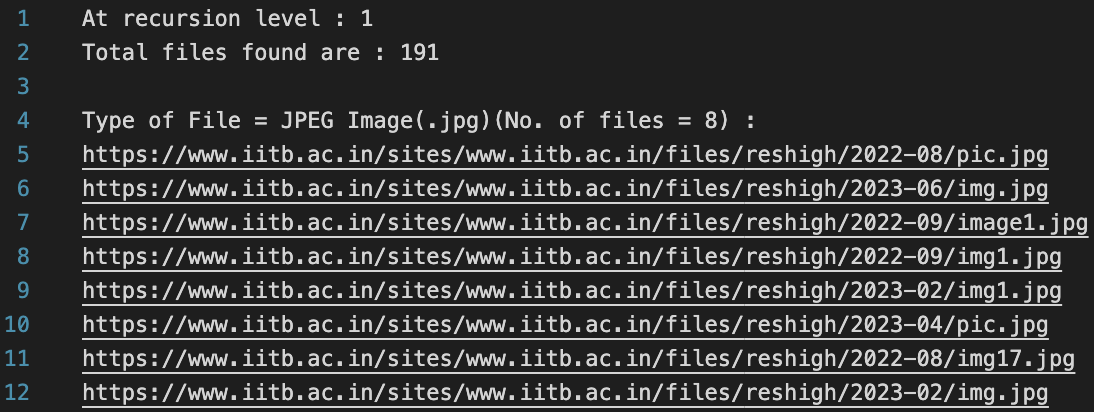
\includegraphics[width=14cm]{output.png}
\begin{itemize}
    \item \textbf{Depth level :}\\[0.4cm]
    The first line shows the Recursion Threshold given to it by user on the command line
    \item \textbf{Total count :}\\[0.4cm]
    The second line shows the total number of unique links printed in the output
    \item \textbf{Type of file and No.of Files :}\\[0.4cm]
    This is the 4th line here,it gives the type of file based on the extension of URL and the no.of such files
    \item \textbf{Links :}\\[0.4cm]
    Finally, These are the links we have successfully crawled, \textbf{Hurray!}\\[1cm]
\end{itemize}
\subsection{custom=1}
This customisation just prints all the links together without any segregation.
\newpage
\subsection{custom=2}
This customisation prints Internal and External Links separately.\\
This is executed by checking the domain of every link using \textbf{urlparse} function\\[1cm]
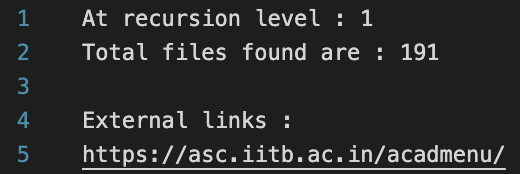
\includegraphics[width=14cm]{external.png}\\[1cm]
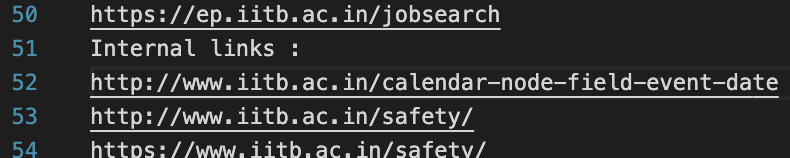
\includegraphics[width=14cm]{internal.png}
\subsection{custom=3}
    This customisation prints links Depth-wise(i.e if we give \textit{\textbf{Threshold value = 3}} then the code executes and finds out what links and obtained at \textit{\textbf{depth = 1}}, print them and then it prints unique links found at \textit{\textbf{depth = 2}} and then same for \textit{\textbf{depth = 3}}.\\[1cm]
    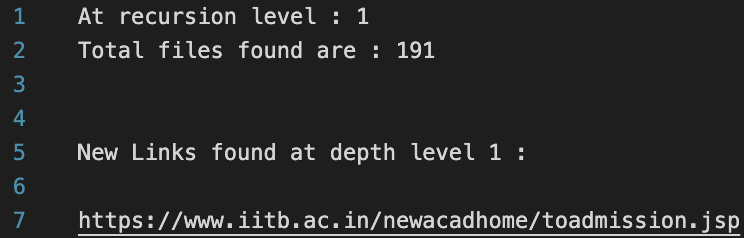
\includegraphics[width=14cm]{depth.png}\\[0.3cm]
    This is achieved by making a dictionary with keys as depth and values as empty sets to which we add the links as there being recursively crawled and later while printing/saving the output, we would uniquely print the links
\section{Error Handling and Changes made from the Base Code}
\subsection{urllib3.disable\_warnings}
\textbf{First Occurrence : Line 15}\\[0.4cm]
If we verify SSL certificate for every link then some websites like \textit{\underline{http://www.iitb.ac.in}} do not give a result,as we are just crawling and printing the resulting links,we don't have to verify certificate but if we don't verify it,some warnings are floated,to neglect them we use the \textbf{urllib3.disable\_warnings} function.
\subsection{Redirecting links}
\textbf{requests.get()} automatically handles redirection and doesn't require us to explicitly add \textit{allow\_redirects}
\subsection{Handling internal referencing}
The below code snippet handles links with \# ,which are included in fragment section of \textbf{urlparse}. These links are not unique webpages rather they just reference a part of the same webpage\\[1cm]
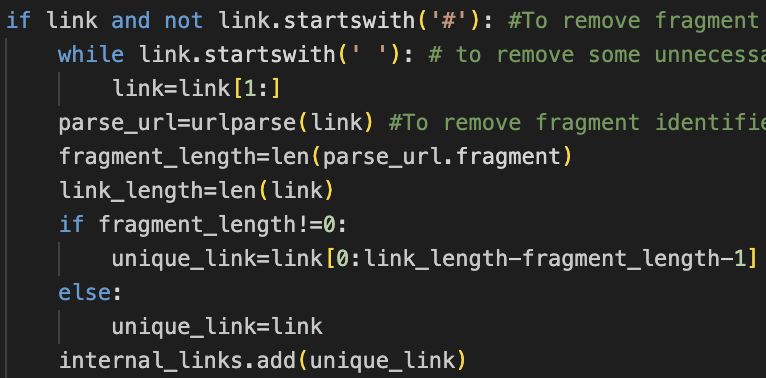
\includegraphics[width=14cm]{reference.png}\\
\cite{link1}
\cite{link2}\cite{link3}\cite{link4}\cite{link5}
\printbibliography
\end{document}
